%chapter_cacop_begin
\graphicspath{ {../body/cacop_figures/}}
%\chapter{基于多媒体特性的呼叫接纳控制算法研究}
\label{chap_cacop}

从目前无线网络的发展情况看,多媒体数据业务将会逐渐取代目前无线通信中话音业务为主的状况。
为此,无线通信标准中的定义中已经开始支持这些多媒体业务的传输。例如,IEEE802.16定义了多媒体数据的调度类型。
本章首先研究和提出针对不同业务类型服务质量的归一化定义。
然后根据这一定义提出了以系统服务质量最优的呼叫接纳控制原则及其相应的接纳控制算法。

\section{前言}
呼叫接纳控制本质是一个管理呼叫连接并进行资源分配与管理的技术。
这项技术以往常常在无线话音网络,如GSM网络,或VoIP(Voice over Internet Protocol)的网络中使用\cite{Perros1996}\cite{Mase2004}。
有时,它也会应用到视频通信的网络中,用来保证连接的视频质量\cite{Systems_2001}\cite{Y-G-Fang.TVT.2002}\cite{Y-Xiao.IEICE.TC.2001}。
通常,它也被看作是在有限的无线频谱资源与大量的资源需求之间的折衷的策略。
比如,在电话服务网络中,由于业务对数据延时的敏感性,使得呼叫接纳控制单元,为了避免网络数据的拥塞不得不拒绝一些连接的接入。
如果在这些情况下不采取相应的措施,网络的状况会发生拥塞甚至恶化。
另外,呼叫接入控制还间接影响着网络资源的分配与管理。
例如,当某一个连接的数据流过于贪婪,占用了大量的网络资源时,
它会造成其它连接的业务服务质量下降,使得网络不得不阻塞新的连接进入或是导致现有连接的中断。
这都将使得网络服务的用户的满意度下降。

近此年来,研究人员提出许多呼叫接纳控制的算法或方案。
有些算法是根据基本的网络性能参数直接用来建立呼叫接纳的准则。这此参数包括比如带宽资源利用率、单位时间内的数据包的个数或在线的呼叫个数等。
当这些参数的值达到或超过了预先设置的上限或是下限,新的呼叫将会被迫延迟接入或是拒绝接入\cite{Y-Qian.TWC.2006} \cite{G-Djuka.TELSIK.2007}。
还有些是将一些底层(物理层或MAC层)的参数加以合并建立基于交叉层的新准则来应用来呼叫接纳控制算法。
例如,学者Song和Zhuang引入了一个被称之SRPT(shortest remaining processing time)的服务准则 \cite{Song2009}。
一个时间窗的大小被设置到一个合适的阈值来判断连接或呼叫是否被接入网络。
学者Yilmaz 和 Chen 也提出了一个类似的思想\cite{Yilmax2009}.
在这篇文献中,他们将资源标上价格并设置价格的阈值。
这种竞价方案是通过分析一个或多个数据流的特点来完成。
最后提出的接纳控制方案使用一个或是多个混合分区的价格阈值,并且周期地对资源进行定价来使系统的效用最大化。
那些不能负担资源费用的用户会被系统拒绝服务。
学者Zhai和Ni提出一个半马尔可夫决策过程来描述呼叫接纳过程 \cite{Zhai2005,Ni2009}。
他们通过把呼叫过程转化为一个求解系统资源利用最大化的数学问题。
学者Zhai和Xiang提出一个信道繁忙率(channel busyness ratio)的概念。
通过检测信道繁忙率来为呼叫接纳提供判断的准则 \cite{Zhai_Chen_Fang_2006}。
还有的学者是通过资源预留的方法来解决呼叫接纳的问题。
例如,Chen和Kuo提出通过动态指派优先级的方法来接纳呼叫 \cite{Chen_Kumar_Kuo_2003,Chen_Kuo_2004}。
学者Elsayed等将三种比例预留的策略:统一预留、容量比例预留和剩余比例预留做了详细的评估\cite{Elsayed02performanceevaluation}。
学者El-Kadi提出的动态预留的方法 \cite{EL-Kadi2002}。
这种方法引入用户数据在短时间内可以容忍通信质量一定程度上的下降,并且基于此提出“借和还”的比例预留方法。
此方法与我们将在本章提出的方法有些类似,所以本章仿真实验中当作对比实验。

以往的这些接纳控制方案中所涉及的测量参数大多都集中在物理层和MAC层上,很少从用户应用的角度来思考呼叫接纳控制。
这主要有两个原因:一个是以前的无线网络承载的业务基本上以话音为绝大多数。其它的业务量极小。
二是尽管可以用交叉层技术使得网络底层得到上层如应用层的流量信息,但是这样会破坏无线网络的分层结构。
所以交叉层技术的应用范围局限性较大。
因此要寻求其它的途径来完成这一任务。
本章的贡献就在于此。
本章首先构造一个简单的服务质量评估模型,将应用层信息与底层参数信息做一个适当的映射关系。
然后,将此模型应用于接纳控制及资源分配,可以在兼顾资源利用效率的情况下,又可保证终端用户所感受到的服务质量。
%
\section{MAC层业务调度类型分类}
随着网络业务的发展,无线通信标准也开始关注业务的种类对通信质量的影响。
譬如,在WiMAX(Worldwide Interoperability for Microwave Access)中,
标准的制定者对MAC层数据包做了初步的分类。
他们把数据分为五类:
每一类业务类型有自己相应的服务质量参数,例如延迟、抖动、丢包或错包率等等。
每一类数据的调度算法都应尽可能满足这些服务质量参数\cite{Tsagkaris_Demestichas_2009}\cite{Andrews_Ghosh_Muhamed_2007}。
%但是同时,我们也注意到WiMAX的标准仅仅将这些数据分类而已,并没有说明如何调度这些已经分类的数据。这也给学者留下一块研究的空间。
此处我们也参照着WiMAX标准定义,将业务分成以下几类。

\begin{itemize}
\item UGS( unsolicited grant service)业务:这种业务类型是指具有实时性要求的业务。
    它的数据具有是周期性产生、包长固定的特点。
    比如T1、E1以及没有静默压缩的VOIP等就属于此类业务。
    这个特点使得UGS业务的数据流比较稳定,突发性较差。
\item rtPS(real-time polling services)业务:这类业务也是具有实时性要求,
    但是与UGS业务不同,它的数据包一般是变长的,同时也具有周期性。
    这类数据包的包头也比UGS数据包的包头要大。
    例如象MPEG(Motion Pictures Experts Group)视频或H.264视频流。
    在调度此类数据时,采用基站指导下移动台单播轮询策略(unicast polling)。
    基站需要通过提供足够多的轮询次数来保证业务的实时性要求。
\item nrtPS (non-real-time polling services)业务:
    这种业务与rtPS业务十分类似。但是它采用的是移动台竞争轮询策略(contention-based polling)。
    如果在竞争轮询期间此类用户很多,就会出现资源申请冲突和后续的冲突避让方案。
    所以,这种方式会引入较大的时间延迟。
\item BE (best-effort)业务:
    此类业务对服务质量的要求在五种业务类型中最低。往往也没有十分具体的QoS指标要求。
    如果能够申请到资源,就进行数据发送。如果不能,则继续等待下一次的调度。
    一般我们把普通的文字网页浏览,或是FTP文件的传送归于此类。
\item ertPS(extended real-time polling service)业务:
    这种业务类型是将上行数据链路的传输协议做了复用。
    在传数据的同时,也可进行无线资源的申请。
    这样可以保证数据量波动较大的情况下,资源能够得到及时的调度。
\end{itemize}

\section{呼叫接纳控制模型与业务流的QoS分析}
\label{sec_qos_metric}
因为不同的业务数据对服务质量的要求差别很大,所以要设计相应的传输机制来应对这种变化。
本节我们将详细描述如何将接纳控制方案与资源分配方案相结合。

%CAC
\subsection{呼叫接纳控制模型}
\label{sec_sec_model}
前面我们提到,呼叫接纳控制的方案就是为了避免网络拥塞,决策某一个呼叫或连接通信服务是否被中断或拒绝。
(因为呼叫一般专指话音通信,所以为避免文字概念混淆,下文一律用“连接”一词来代替“呼叫”一词。)
此处,我们假设一个一般的呼叫接纳控制的网络模型。
在此模型中,有一个基站和~$K$~连接,如\figref{fig_system_model_cac}所示。

其中包括已经在线的$K-1$个连接和$1$个正在申请进入的新连接。
这些连接根据不同的业务种类被分为五种类型,UGS,rtPS,nrtPS,BE和ertPS。
在第$K$个连接被接入之前,所有 ($K-1$) 连接共享基站所提供的带宽资源,记为$B_{total}$。
当第$K$个连接进入基站的覆盖范围,并提交进入和资源分配的申请后,系统触发一次接纳控制的判断过程。
首先,服务质量评估单元(QoS Evaluator)会根据目前的连接情况,提交一份带宽资源分配的方案,记为向量 $\mathbf{b}$ 。
其中,$b_i$ 表示第$i$个连接所分配到的带宽,那么,$\mathbf{b} = [ b_1, b_2, b_3, \dots, b_K]$ ,而且 $\sum_{i=1}^K b_i \le B_{total}$。
然后,
基于这个方案 $\mathbf{b}$,接纳控制单元(Call Admission Control)根据每一个连接所分配到的带宽 $b_i$来评估每一个连接的QoS水平和整个系统的QoS水平。
最后,接纳控制单元再决定接受或拒绝这个连接的进入请求。
%%
\begin{figure*}[t]
\centering
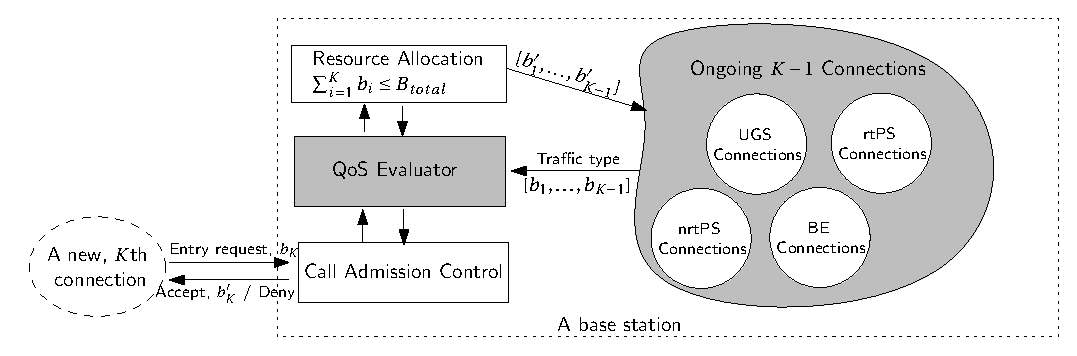
\includegraphics[width=0.95\textwidth]{cacop_qos_model_system.eps}
\caption{ 呼叫接纳控制的系统模型} \label{fig_system_model_cac}
\end{figure*}
%%%%%%
%QoS Metric
\subsection{带宽分配与QoS之间关系分析}
在以往的大多数文献中,接纳控制的QoS已经做了许多重要的研究工作。
他们对用户或系统的QoS评价指标一般直接从网络底层,如物理层或MAC层,直接获得。
譬如,带宽资源的利用率、掉话率或呼叫中断概率等等。
经过分析,我们认为,因为通信网络是以用户服务为中心的,而且用户一般只能从网络应用层感知QoS;
所以,对于业务连接的QoS评价也应该最好从应用层来评价。
但是,由于目前的通信网络是基于分层结构设计原则,上层的信息如果需要传递新的信息,就要重新修改和制定分层的协议。
这对目前通信网络的构造冲击太大,会造成网络的大规模的改造,显得不太切合实际情况。
因此,
我们提出通过一个预先认定的服务质量QoS的映射模型,利用底层所能获得的参数信息将上层QoS的估计出来,
就可以最大程度地兼容现有的通信网络。
对于在线业务连接而言,最重要的网络参数就是它们所分配到的带宽资源 $\mathbf{b}$。
我们提出服务质量的评估应该把带宽资源与业务同时包括在内。
下面,我们结合业务类型,对带宽资源对各项业务服务质量的评估影响做详细的介绍。

\begin{enumerate}[(1)]
    \item UGS业务与QoS评价:
        话音业务是UGS业务中最典型的一种。
        E模型(E-Model)提供了一种可以客观评价话音传输服务质量的方法 \cite{ITU:G107}。
        此模型通过提取网络参数(如延时或丢包)定义了对话音评估的分析模型。
        E模型可以使用R因子(R-factor)来评价话音质量。R因子的值域在$0$到$100$之间。
        $0$表示质量最差;$100$表示话音质量最好。有时,R因子会简化为一个更常用的评价指标MOS(Mean Opinion Score)。
        MOS用$1$到$5$来评价话音质量。$5$表示最好的质量,$1$表示最差的质量\cite{NK:IEICE:2005}。

        R因子的值可通过下面\eqref{eqn:chap_cacop:FactorR}计算得到:
\begin{equation}
\label{eqn:chap_cacop:FactorR}
R = R_0 − I_s − I_d − I_e + A 
\end{equation}
其中,$R_0$ 表示基本的信噪比(signal-to-noise ratio)。
$I_s$ 表示对于话音信号的损失之和。
$I_d$ 表示延时对通信的损害。
$I_e$ 表示由于低码率的编码方式对话音质量的影响。
$A$ 表示一个优势因子(advantage factor),表示用户的容忍度。
为了计算方便,\eqref{eqn:chap_cacop:FactorR} 可以改写为\eqref{eqn:chap_cacop:FactorR_simple}
\begin{equation}
R = 93. 4 - I_d ( T_a ) -I_e ( codec, loss )
\label{eqn:chap_cacop:FactorR_simple}
\end{equation}
其中,$I_d$是一个单程延时函数。
(这里,我们假设延时较小可以被忽略。)
$I_e$ 代表编码器的类型及丢包情况。
我们通过E模型计算器来得到不同的丢包状况下的话音质量R因子的值\cite{ITU:EModel:Caculator}。 
结果如表\ref{tb:R_factor}所示。
从表中数据可以看出,话音业务对带宽资源极为敏感而且对丢包容忍度较低。通常R因子如果小于$50$则表明话音质量很差,用户不满意。


\begin{table}[tb]
%\caption{R-Factor vs. Packet Loss} \label{tb:R_factor}
\caption{R因子与丢包率} \label{tb:R_factor}
\begin{center}
%\footnotesize
\begin{tabular*}{0.7\textwidth}{lcccccccccccc}
%\begin{tabular*}{0.5\textwidth}{lp{9mm}}
\toprule 
丢包率(\%):& 0& 0.1& 0.3& 0.5& 0.7& 0.9& 1& 2\\
R-因子: &93.2& 84.6& 71.3& 61.5& 54.1& 48.2& 45.2& 29.9\\ 
\bottomrule
\end{tabular*}
\end{center}
\end{table}

综上所述,我们定义UGS业务的服务质量评估公式,如\eqref{eqn:chap_cacop:metric_voice}所示。
\begin{equation}
\label{eqn:chap_cacop:metric_voice}
\alpha^{UGS}=
\begin{cases}
1 & \text{if $b=B$,}\\
0 &\text{others}
\end{cases}
\end{equation}
其中,$\alpha^{UGS}$ UGS业务流的服务质量QoS的值。
$b$是所分配到的带宽;
$B$是对应于此话音业务需要,其申请的带宽资源数量。
为了表示简单起见,
我们改写为如下形式,
\eqref{eqn:chap_cacop:Dirac_UGS}.
%
\begin{equation}
\label{eqn:chap_cacop:Dirac_UGS}
\alpha^{UGS}= \delta_{b}(B) = 
\begin{cases}
1 & \text{if $b= B$,}\\
0 &\text{others}
\end{cases}
\end{equation}
\item rtPS业务与QoS评价: 
视频业务是一种典型的rtPS应用。
在视频传输或编码应用中,峰值信噪比 ( peak signal-to-noise ratio,PSNR)是最常见视频质量评价的方法。
它所采用的方法是将原始图像$I$与受损的重建图像$K$之间做逐像素的比较,
如\eqref{eqn:chap_cacop:psnr}所示。 
%
\begin{align}
\label{eqn:chap_cacop:psnr}
& PSNR = 10 \cdot \log_{10} \left( \frac{MAX_I^2}{MSE} \right)
\end{align}
其中,$MAX_I$ 是单个像素值域中的最大值。
如果是每个像素点用$8$个比特表示,那么这个值就是$255$。
更一般的情况,如果采用每个像素用$z$个比特表示,那么 $MAX_I$就为 $2^z - 1$. 均方误差(mean squared error,MSE)的定义为\eqref{eqn:chap_cacop:mse},它用来表示原始图像$I$与解码重构图像$K$之间差。
\begin{align}
\label{eqn:chap_cacop:mse}
MSE = \frac{1}{MN} \sum_{i=0}^{M-1}\sum_{j=0}^{N-1} \left[I(i,j) - K(i,j)\right]^2 
\end{align}
PSNR在视频编码解码研究领域广泛使用。
然而,它不能直接在通信网络的MAC层中接纳控制单元中使用。
因为,如果要想得到PSNR的值,首先要对压缩视频解码,恢复为YUV的图像帧。
这就意味着在MAC层中要嵌入视频解码单元,这一要求不太现实。
其次,还要有参考的视频帧。它是指原始未压缩的视频。
在一个通信网络中,这些数据对于接纳控制单元而言是不可能提前得到的。
那么,类似于UGS业务连接,我们一般所能得到的信息只能是带宽分配情况$b$,以及业务连接对所需带宽的申请情况$B$。

最简单的情况下,我们可以类比网络吞吐量的比值,将$\frac{b}{B}$当做是评估视频连接的QoS。不幸的是,视频质量与比值$\frac{b}{B}$并不是简单的线性关系
 \cite{He1013856}。
我们要寻找别的替代方案。这个替代方案要能够反应出服务质量与视频质量PSNR的关系,又能在MAC层中方便地实现。
我们发现,率失真优化(rate distortion optimization,RDO)思想可以应用到我们的问题中。
率失真优化是一种研究码率与压缩视频质量关系的方法
\cite{He1013856}\cite{E-H-Yang.TIP.2007} \cite{J-Y-Liu.ICIP.2009} 。
这种方法的目的是要建立视频的失真(损失)与所分配的码率之间的关系模型。
通过考察这个模型来对编码的码率做出指导。
从资源分配的角度看,视频质量与带宽分配之间的存在着紧密的联系。
为了能够找到一个合适的模型来描述视频质量与带宽分配之间的关系,我们构造与比较了一些典型的拟合模型,结果如表\ref{tb:chap_cacop:fit_functions} 如示。
\begin{table}[tb]
\caption{拟合模型} 
%\caption{Fitting Model Types} 
\label{tb:chap_cacop:fit_functions}
\centering
\begin{tabular}{llcc}
\toprule
ID& $f(x)$ & SSE & Adjusted R-square\\
\midrule
1&$ae^{bx}$ & 594.8 &0.4233\\
2&$p_1 x + p_2$ & 505.7 & 0.5096\\
3&$a_1e^{-((x-b1)/c1)^2}$&339.1&0.6243\\
4&$a_0 + a_1\cos(xw) + b_1\sin(xw)$&217.5&0.7317\\
5&$p_1x^2 + p_2x + p_3$ &207.5 & 0.7701\\
6&$p_1x^3 + p_2x^2 + p_3x + p_4$&62.04&0.9465\\
7&$a(1-e^{ \rho \frac{x}{\max(x)}})$ &19.83 & 0.9808\\
8&$p_1x^4 + p_2x^3 + p_3x^2 + p_4x + p_5$&14.93 &0.9871\\
\bottomrule
\end{tabular}
\end{table}
表中的数据显示了不同拟合函数模型下,对视频测试序列“Forman”的拟合结果。
从表中的结果可以看到,函数模型$7$和$8$性能明显优于其它模型。
如果我们从数学的拟合效果(SSE 和Adjusted R-square)来考虑,模型$8$ ($p_1x^4 + p_2x^3 + p_3x^2 + p_4x + p_5$)会更准确。
但是,此处我们选择模型 $7$,$a(1-e^{ \rho \frac{x}{\max(x)}})$。 
选择它原因有三个:
一是,多项式模型保用了较多的系数来描述视频的特性。
而指数模型只有一个系数$\rho$来描述业务的特性。从模型的简洁程度来看,
指数模型更简单。
二是,指数模型尽管不如多项式模型$8$,但是它远优于其它的函数模型。
这里我们在简洁与准确性之间做了适当的折衷。
三是,指数模型可以涵盖其它类型的业务。这样我们可以用统一的模型来表达多种业务的服务质量,下面小节中我们会详细解释。

为了表示方便起见,我们将指数模型进行归一化的处理,如
\eqref{eqn:chap_cacop:qos_level_users}所示。
\begin{equation}
\alpha^{rtPS} = \frac{PSNR_b}{PSNR_B} \approx \frac{1- e^{-\rho \frac{b}{B} }}{1-e^{-\rho}}, \rho > 0
\label{eqn:chap_cacop:qos_level_users}
\end{equation}
其中,
$\alpha^{rtPS}$ 表示归一化后的视频流或rtPS数据流的服务质量。
$PSNR_b$ 和 $PSNR_B$ 分别表示编码的码率为$b$ 和 $B$的视频质量。
$\rho$ 代表 rtPS连接的数据流特征值。
每一个rtPS都会自己的特征值$\rho$。我们假定它在传输之前可以确定下来。
$b$表示
$e^{-\rho \frac{b}{B}}$部分表示失真。
$1- e^{\rho \frac{b}{B}}$ rtPS连接的QoS值。
分母$1-e^{-\rho}$是用来做归一化处理的。
$b$ 表示当前连接所分配到的带宽数量,并且要求它大于它的最低带宽要求$B_{\min}$。
$B$表示当前连接要求的带宽数量。
为了进一步验证此模型有效,我们对不同标准视频序列按不同码率编码,结果如 \ref{fig:chap_cacop:qos_rate_cac}所示。
为了比较,我们在结果图中增多一条$\rho=4$的曲线。
从结果的各条曲线可以看到,所提出的以带宽参数值$b,B$及业务特征值$\rho$为基础的服务质量评估的模型可以做为rtPS或视频连接的服务质量的估计。
\begin{figure}[tb]
\begin{center}
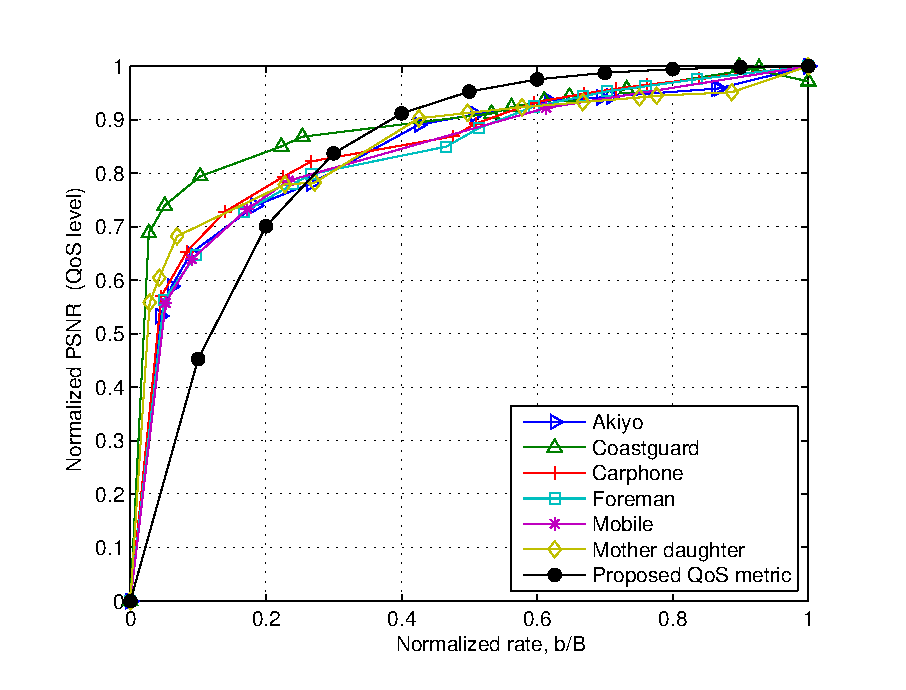
\includegraphics[width=0.75\textwidth] {cacop_qos_rate_cac.eps}
\end{center}
\caption{视频连接PSNR与码率的关系} 
\label{fig:chap_cacop:qos_rate_cac}
\end{figure}

\item 其它类型业务与QoS评价
对于BE类型的业务,网页浏览HTTP应用或文件传输FTP应用是典型的例子。
HTTP(Hypertext Transfer Protocol)是互联网数据传输中最重要的应用层协议之一\cite{Fielding_1999}。 
由于其简捷、快速的方式特点,适用于分布式超媒体信息系统。
FTP是用于在网络上进行文件传输的一套标准协议。它属于网络协议组的应用层。用于Internet上的控制文件的双向传输。
同时,它也是一个应用程序(Application)。用户可以通过它把自己的PC机与世界各地所有运行FTP协议的服务器相连,访问和下载服务器上的大量程序和信息 \cite{Postel_Reynolds_1985}。
这两类业务应用的共同点是对用户对服务质量的要求取决于在发送端发送数据的总量与接收端已接收数据量的多少。
所以,我们把这类应用的服务质量简单地定义为,如\eqref{eqn:chap_cacop:BE_metric} 所示。
%
\begin{equation}
\label{eqn:chap_cacop:BE_metric}
\alpha^{others} = \frac{b}{B}
\end{equation}
%
其中,$b$是分配得到的带宽资源,$B$是对于BE类应用而言所需的带宽资源。
它们的比值就可以表示这类应用连接的服务质量水平。
对于最后两类业务nrtPS与ertPS,我们假定他们的业务与BE的类型类似,也用 \eqref{eqn:chap_cacop:BE_metric} 表示。
\end{enumerate}

综上所述,因为各类业务的服务质量的计算公式差别不大,下面我们将它们总结一下。
我们注意到\eqref{eqn:chap_cacop:qos_level_users}在业务特征值$\rho$趋向于无穷大时存在极限,且恰是BE业务的服务质量计算公式。
%
\begin{equation}
\label{eqn:BE_limit}
\lim\limits_{\rho \to 0 } \frac{1- e^{-\rho \frac{b}{B} }}{1-e^{-\rho}} = \frac{b}{B}
\end{equation}

所以将\eqref{eqn:chap_cacop:BE_metric}其可以改写为\eqref{eqn:chap_cacop:BE_metric_2}
%
\begin{equation}
\label{eqn:chap_cacop:BE_metric_2}
\alpha^{others} = \frac{b}{B} = \frac{1- e^{-\rho \frac{b}{B} }}{1-e^{-\rho}} \quad \text{if} \quad \rho \to 0
\end{equation}
%
最后我们将各种业务类型的服务质量评估公式整理可得 \eqref{eqn:chap_cacop:alltype_metric}
%
\begin{equation}
\alpha = 
\begin{cases}
\delta_{b}(B), &\text{for UGS traffic} \\
\frac{1- e^{-\rho \frac{b}{B} }}{1-e^{-\rho}}, \rho > 0& \text{for rtPS traffic}\\
\frac{1- e^{-\rho \frac{b}{B} }}{1-e^{-\rho}}, \rho>0, \rho \to 0, &\text{for BE, nrtPS, ertPS traffic}\\
\end{cases}
\label{eqn:chap_cacop:alltype_metric}
\end{equation}
\section{资源分配的优化分析}
接纳控制的本质是为了保证各个连接的通信服务质量,防止新连接占用资源后对在线连接产生负面的影响。
一个好的接纳控制方法应该在充分利用资源的前提下,使用户的服务质量最大化。
这个问题可归结为如下的一个优化问题。
假设在系统中有$M$个 UGS连接,$N$个 rtPS 连接和 $Q$个其它类型的连接,而且,这些连接之间是彼此无关的。
那么所有连接的QoS之和可以表示为基站的效用,如\eqref{eqn:chap_cacop:bs_qos} 所示。
\begin{align}
U_{BS} &= \displaystyle \sum_{i=1}^K \alpha_i \nonumber \\
&= \sum_{i=1}^M\alpha_i^{UGS} + \sum_{i=1}^N\alpha_i^{rtPS} + \sum_{i=1}^Q\alpha_i^{others} \nonumber \\
&=\displaystyle M^\prime + \sum_{i=1}^N \left( \frac{1- e^{-\rho_i^r
\frac{b_i}{B_i} }}{1-e^{-\rho_i^r}} \right)
 + \sum_{i=1}^Q \left( \frac{1- e^{-\rho_i^o
\frac{b_i}{B_i} }}{1-e^{-\rho_i^o}} \right),
\label{eqn:chap_cacop:bs_qos}
\end{align}
其中,$M^\prime(\le M)$ 表示$M^\prime$ UGS连接分配到了所需的带宽资源。
$\rho_i^r$ 是第$i$个rtPS连接的数据流特征。 
$\rho_i^o$ 表示BE类型的连接特征。此处我们假定这个很小且接近于零。
为了表示方便,我们用符号$\rho_i$来统一表示$\rho_i^r$ 和$\rho_i^o$。
$U_{BS}$ 表示基站在给$K$个连接提供服务所能收获的效用。
如果$U_{BS}$有最大值, 那么一定存在一个资源分配的优化解
$\mathbf{b}$ 。
我们会把这个解做为接纳控制的判决条件。
因此,这个优化问题可定义为如下形式。
\begin{align}
\mathbf{b}^* &= \arg \max \left\{ U_{BS}(\mathbf{b}) \big| \mathbf{b} = [b_1, b_2, \dots, b_K] \right\} \label{eqn_u_bs_qos}\\
&\text{subject to:}\nonumber\\
&\displaystyle\sum_{i=1}^{K}b_i + B_{ava}= B_{total} \nonumber
\end{align}
其中, $\mathbf{b}^*$ 是资源分配的优化解。
$B_{total}$ 是系统所能提供的全部带宽。
$ B_{ava} $是剩余的带宽资源。

因为接纳控制通常是在业务负载大的情况下产生作用,所以为了简单起见,
我们剩余资源为零。同时,因为UGS类型的连接对带宽的要求严格,所以这些连接必须按照申请的数量分配。
我们则将上面的优化问题改写为 \eqref{eqn:chap_cacop:final_opt_qos}
\begin{align}{}
\label{eqn:chap_cacop:final_opt_qos}
\mathbf{b}^* &= \arg \max \left\{ U_{BS}(\mathbf{b}) \big| \mathbf{b} = [B_1, B_2, \dots,B_M,\right.
 \left. b_{M+1}, \ldots, b_K] \right\} \\
&\text{subject to:}\notag \\
&\sum_{i=1}^M B_i + \sum_{i=M+1}^{K}b_i= B_{total} \notag
\end{align}

下面我们来解这个优化问题。
先说明这个优化问题存在解。
为了方便书写,引入一个新的变量$x$来表示$\frac{b}{B}$。
\begin{equation*}
\begin{split}
x_i = \frac{b_i}{B_i} , i \in [M+1, K].
\end{split}
\end{equation*}
我们引入拉格朗日乘子$\lambda$,然后写出所需的拉格朗日方程,如
\eqref{eqn:chap_cacop:lagrange_defination}.
%%%
\begin{align}
&\displaystyle F(x_{M+1}, x_{M+2}, \dots, x_K, \lambda)= \sum^{M+N}_{i=M+1}
\left( \frac{1-e^{-\rho_i x_i}}{1-e^{-\rho_i}} \right) \nonumber \\
& \qquad \displaystyle +\sum_{i=M+N+1}^K\left( \frac{1-e^{-\rho_i x_i}}{1-e^{-\rho_i}} \right) 
 + \lambda
\left(B_{total} - \sum_{i=1}^M B_i -\sum^K_{i=M+1} x_i B_i \right).
\label{eqn:chap_cacop:lagrange_defination}
\end{align}
%%%
而后,对上面方程求两阶导数$\frac{\partial ^2F}{\partial x_i \partial x_j}$得Hermitian矩阵${M}$.
%%%
\begin{eqnarray*}
{M} = & 
\left[
\begin{array}{cccc}
\frac{\partial ^2F}{\partial x_{M+1} ^2} &\frac{\partial ^2F}{\partial x_{M+1} \partial x_{M+2}} & \dotsi & \frac{\partial ^2F}{\partial x_{M+1} \partial x_K} \\
\frac{\partial ^2F}{\partial x_{M+2} \partial x_{M+1}}& \frac{\partial ^2F}{\partial x_{M+2} ^2}& \dotsi & \frac{\partial ^2F}{\partial x_{M+2} \partial x_K}\\
\vdots & \vdots & \ddots & \vdots \\

\frac{\partial ^2F}{\partial x_{K} \partial x_{M+1} } &\frac{\partial ^2F}{\partial x_{K} \partial x_{M+2}} & \dotsi&\frac{\partial ^2F}{\partial x_K ^2}\\
\end{array}
\right] \\
=&
\left[
\begin{array}{cccc}
\frac{-\rho_{M+1}^2 e^{-\rho_{M+1} x_{M+1}}}{(1-e^{-\rho_{M+1}})} & & & \text{{\huge{0}}}\\
&&\ddots\\
\text{{\huge{0}}} &&& \frac{-\rho_{K}^2 e^{-\rho_{K} x_{K}}}{(1-e^{-\rho_{K}})}\\
\end{array}
\right] 
\end{eqnarray*}
很明显,如果$\rho >0$ 那么$1-e^{-\rho} >0$。
矩阵${M}$是负定的(negative-definite)。
因此对于BS的效用$U_{BS}$来说,存在局部极大值点。
下面我们来具体求解这个问题。
首先让对方程两连求一阶导数,并置为零,
$dF = 0$,则有下面一系列等式。
%%%
\begin{subequations}
\label{eqn_derivate}
\begin{align} &\frac{\partial F}{\partial x_{M+1}} =
\frac{\rho_{M+1} e^{-\rho_{M+1} x_{M+1}}}{(1-e^{-\rho_{M+1}})} - \lambda B_{M+1} = 0 \tag{\theequation -M+1}\\
&\frac{\partial F}{\partial x_{M+2}} =
\frac{\rho_{M+2} e^{-\rho_{M+2} x_{M+2}}}{(1-e^{-\rho_{M+2}})} - \lambda B_{M+2} = 0 \tag{\theequation -M+2}\\
\nonumber & \qquad \vdots \qquad \vdots \qquad \vdots \\
&\frac{\partial F}{\partial x_K} =
\frac{\rho_K e^{-\rho_K x_K}}{(1-e^{-\rho_K})} - \lambda B_K = 0 \tag{\theequation -K}\\
&\frac{\partial F}{\partial \lambda} = B_{total} - \sum_{i=1}^M B_i -
\sum^K_{i=1}x_iB_i = 0 \tag{\theequation -K+1}
\end{align}
\end{subequations}
%%%
根据公式 (\ref{eqn_derivate}),我们有
%%%
\begin{equation*}
\begin{split}
&\frac{\partial F}{\partial x_i} = \frac{\rho_i e^{-\rho_i
x_i}}{(1-e^{-\rho_i})} - \lambda B_i = 0\\
%\implies &\rho_i e^{-\rho_i x_i} =\lambda B_i(1-e^{-\rho_i})\\
%\implies &\ln\rho - \rho x_i = \ln [\lambda B_i (1-e^{-\rho_i})]\\
\implies &x_i = \frac{1}{\rho_i} \ln \left[ \frac{\rho_i}{\lambda B_i(1-e^{-\rho_i})} \right] \\
\end{split}
\end{equation*}
%%

再将 $x_i$ 代入公式 (\ref{eqn_derivate}-K+1),则又有
%%%
%
\begin{equation}
\begin{split}
&B_{total} -\sum_{i=1}^MB_i = \sum_{i=M+1}^K x_i B_i \\
&= \sum_{i=M+1}^K \frac{B_i}{\rho_i} \ln \left[ \frac{\rho_i}{\lambda B_i(1-e^{-\rho_i})} \right] \\
%&= \sum^K_{i={M+1}}\left[- \frac{1}{\rho_i}\ln \lambda - \frac{1}{\rho_i}
%\ln (B_i) - \frac{1}{\rho_i} \ln (1-e^{-\rho_i}) + \frac{1}{\rho_i}
%\ln
%\rho_i \right] B_i\\
%&= \sum^K_{i={M+1}}\left[- \frac{B_i}{\rho_i} \ln \lambda -
%\frac{B_i}{\rho_i} \ln (B_i) - \frac{B_i}{\rho_i} \ln (1-e^{-\rho_i})
%+ \frac{B_i}{\rho_i} \ln
%\rho_i \right]\\
%&= -{\ln \lambda}\sum^K_{i={M+1}} \frac{B_i}{\rho_i} 
%- \sum^K_{i={M+1}} \frac{B_i \ln (B_i)}{\rho_i} 
%- \sum_{i={M+1}}^K \frac{B_i\ln(1-e^{-\rho_i})}{\rho_i} \\ 
%& \hspace{5mm}+ \sum^K_{i={M+1}} \frac{ B_i\ln \rho_i} {\rho_i} \\
\end{split}
\label{eqn_find_mu}
\end{equation}

%%%
基于公式 (\ref{eqn_find_mu}), 我们可以解出$\lambda$.
%%%
\begin{equation*}
\begin{split}
\lambda &= \exp \left( \frac{\sum_{i=M+1}^K \frac{B_i}{\rho_i} \ln \left[ \frac{\rho_i}{B_i(1-e^{-\rho_i})} \right]
}{\sum_{i=M+1}^K \frac{B_i}{\rho_i}} \right.
+ \left. \frac{ 
\sum_{i=1}^M B_i - B_{total}}{\sum_{i=M+1}^K \frac{B_i}{\rho_i}} \right)\\
\end{split}
\end{equation*}
%%%

然后,可以求得
%%%
%
\begin{equation}
\begin{split}
x_i & = \frac{1}{\rho_i} \ln \frac{\rho_i}{B_i(1-e^{-\rho_i})} \\
&-\frac{1}{\rho_i}\left( \frac{\sum_{j=M+1}^K \frac{B_j}{\rho_j} \ln \left[\frac{\rho_j}{B_j(1-e^{-\rho_j})}\right] 
}{\sum_{j=M+1}^K \frac{B_j}{\rho_j}} \right)
-\frac{1}{\rho_i}\left( \frac{ 
\sum_{j=1}^M B_j - B_{total}}{\sum_{j=M+1}^K \frac{B_j}{\rho_i}} \right) \\
\end{split}
\end{equation}
%
%%%

最后,整理可得带宽分配的解。
%
\begin{equation}
\begin{split}
\mathbf{b^*}& = [b^*_{M+1}, \cdots, b^*_{K}]\\
b_i^* & = x_iB_i = \frac{B_i}{\rho_i} \ln \frac{\rho_i}{B_i(1-e^{-\rho_i})} \\
&-\frac{B_i}{\rho_i}\left( \frac{\sum_{j=M+1}^K \frac{B_j}{\rho_j} \ln \left[\frac{\rho_j}{B_j(1-e^{-\rho_j})}\right] 
}{\sum_{j=M+1}^K \frac{B_j}{\rho_j}} \right)
 -\frac{B_i}{\rho_j}\left( \frac{ 
\sum_{j=1}^M B_j - B_{total}}{\sum_{j=M+1}^K \frac{B_j}{\rho_i}} \right), i \in [M+1, \cdots, K] \\
\end{split}
\label{eqn:b_i_bw}
\end{equation}
%
\section{提出的接纳控制算法}
\label{sec_alg}
基于上一节所得到的带宽分配方案,我们提出一个接纳控制算法。
在此算法中,我们假设分配到资源数量应该大于业务所需的最小数量,即
$b_i^* \ge B_i^{\min}$. 
这个最小值与业务的类型相关。不同业务均有所不同。
例如,对于话音应用来说,它所需的带宽的最小值就被设置为它申请值。
对于象视频这样的rtPS应用,一般$b_i>=B_i^{\min}$
对于新用户$K$而言,
如果$b_K^*$ 小于所需的资源的最小值$B_K^{\min}$,系统会拒绝这个连接进入。
因为如果按这样的资源量分配给连接$K$,服务质量会很差,用户肯定不满意。
另外,
在我们的算法,使用了优级的概念。我们假定在线连接的优先级要比新连接的优先级要高。这样的假定会造成在我们的算法中在线用户的通信不会被系统中断。

由于上述的两个假定,我们的算法会在带宽分配的过程中出现迭代。
比如,如果一个在线的连接由分配算法(\ref{xxxx})计算所得的资源数目小于它的最小资源需求数目,我们认为这个连接应该受到保护。
接纳算法会将取消此次计算过程,将此连接和它占用的资源排除在外,
然后再重新启动新一轮的带宽计算过程。
直到不再出现在线连接所分配的资源会小于它最低要求。
对于连接$K$来说,如果最后的结果大于其最低要求,则允许其进入系统;否则,这个连接会被系统阻塞(blocked)。

算法的详细流程如流程{\bf{算法 \ref{agr_cac}}}所示。

\begin{algorithm}[!htpb]
\SetAlgoLined
% assume $B_{ava}=0$\;
等待一个新的连接进入请求\;
新连接$K$申请进入;假定此时系统中有$K-1$连接正在进行通\;
\eIf {$B_K<= B_{ava}$}{
允许连接$K$进入系统,被分配带宽$B_K$\;
}{

Calculate the optimum bandwidth value $\bf b^*$ according to Eqn.(\ref{eqn:b_i_bw}) \;
\If{$b_i^* < B_i^{\min} $}{
The $i$th connection is excluded for the bandwidth allocation this time,
and $B_{total} = B_{total} - b_i^{old}$
, $K = K-1$ \;
{\bf{go to 6}}\;
}
\eIf{$b_K< B_K^{min}$}{
Block the new connection request\;
{\bf{go to 1}}\;
}{
Accept the new connection request\;
\For{$i=1$ \KwTo $K-1$}{
The connections excluded by CAC scheduler keep their original resources.\;
Adjust the bandwidth of connections based on the optimum bandwidth value ${b_i^*}$ \;
}
Allocate the bandwidth $b_K^*$ to the new connection\;
}
}
{\bf{go to 1}}\;
\caption{Proposed CAC scheme} \label{agr_cac}
\end{algorithm}

After a new incoming connection sends its request of entry to a BS, CAC process starts. 
If the BS has the available bandwidth enough for the its demand at that time, the new connection $K$ will be given the access right and its required resource is allocated to it.
Otherwise, the optimum value of bandwidth $\bf{b^*}$ for the connections.
Under a lack of resource, if a connection is accepted, two conditions should be satisfied. 
One is that the value $b_K^*$ is greater than the threshold $B_K^{min}$ for the new connection. 
The other is that allocated bandwidth $b_i^*$ is greater than $B_i^{\min}$ for the ongoing connections. 
After the allocated bandwidth $\bf b^*$ is ready, we adjust allocated bandwidth of other $K-1$ ongoing connections using their optimum values. 
And then we allocate the $b_K^*$ bandwidth to the new connection to the end. 
Thus, we can keep the QoS level of the BS as high as possible all the time. 
The step 7, 8 ,9 mean that we exclude the specific ongoing connection from the process of bandwidth allocation, whose optimal value of allocate bandwidth is less than its lowest limit. 
The iterated bandwidth allocation will not stop until the reminder connections satisfy the conditions, $b_i^* \ge B_i^{\min}$.

%
%%
%%


